\chapter{Desarrollo con tarjetas gráficas}\label{cap3}

\section{Breve historia de la computación con GPUs}

Desde hace bastante tiempo se lleva usando las capacidades de las tarjetas gráficas para realizar computación. Concretamente se han utilizado para la realización de efectos sobre texturas y polígonos con la tecnología denominada \emph{shaders}. Estos \emph{shaders} son pequeños programas que transforman la forma de verse los puntos o como se transforman los polígonos y que se han estado ejecutando en las GPUs para mejorar su rendimiento.

A partir de esta tecnología y tras numerosas especulaciones sobre las capacidades de las tarjetas gráficas para realizar cálculos más genéricos, las compañías empezaron a abrir sus sistemas para permitir cargar códigos orientados a cualquier tipo de cálculo matemático.

Los primeros productos con este tipo de tecnología provinieron de BionicFX y fueron presentados a principios de 2005 \cite{website:extremetech_gpu_audio}. En este caso se hacía uso de gráficas con GPU NVIDIA para procesador de audio. Para ello transformaba el sonido en datos gráficos y luego éstos se procesaban con los medios matemáticos de que disponía la GPU.

Más tarde, en el año 2006, la compañía AMD anuncia la comercialización de AMD Stream Processor~\cite{website:amd_press_stream}, el primer sistema de cálculo basado en tarjetas gráficas. De este modo se empezó a comercializar el primer sistema que realmente permitía cargar código de usuario en la tarjeta para realizar cálculos que no estuviesen directamente relacionados con generación de imagen en 3D.

La compañía NVIDIA publica el 15 de febrero de 2007 la biblioteca CUDA~\cite{website:nvidia_press_cuda} que permite usar sus tarjetas gráficas para cálculo y, además, comercializa la arquitectura Tesla que, como en el caso de ATI, es un sistema específico de cálculo basado en tarjetas gráficas.

En base a esta popularización del cómputo con tarjetas gráficas y por  su utilizad gran utilidad para todo tipo de procesos (especialmente aquellos destinados a multimedia e investigación), Apple publica un borrador de OpenCl (Open Computing Language) y posteriormente éste es pasado a control de Khronos Group~\cite{website:khronos_press_opencl}. OpenCl es  el primer estándar creado específicamente para cómputo distribuido, orientado principalmente a GPUs, y que ofrece una interfaz común para todo tipo de tarjetas gráficas y otros sistemas de cálculo (como procesadores multinúcleo, FPGAs, procesadores CELL, etc.). Esta tecnología solo se incluye de serie en el sistema operativo Apple Mac OS X 10.6, pero fabricantes como ATI y NVIDIA proveen de controladores para otras plataformas.

El mecanismo más eficiente para aprovechar las capacidades de una tarjeta gráfica es utilizar la API del fabricante ya que éste está optimizado para aprovechar mejor la arquitectura. Esto supone que en casos en los que la eficiencia es algo absolutamente crítico sea mejor opción frente al uso de la biblioteca OpenCl.

Estos sistemas están teniendo mucha relevancia debido a su alto rendimiento, especialmente en aplicaciones científicas. Además, se han realizado avances en el desarrollo de aplicaciones específicas de ruptura de contraseñas.

En la actualidad la computación con tarjetas gráficas está empezando a utilizarse en todo tipo de cálculos, tanto para investigaciones científicas  como para herramientas de usuario como descompresores de vídeo y audio, filtros gráficos en herramientas de diseño o videojuegos. Todo esto gracias a las grandes capacidades de paralelización de cálculos de las GPUs como a la facilidad de realizar cálculos vectoriales de forma sencilla. Esto significa que es una tecnología apoyada por la industria y que se va a disponer de soporte y documentación para realizar desarrollos con la misma.

Se puede comprobar, además, como en el año 2008 empezaron a surgir los primeros sistemas orientados a la seguridad informática que se apoyaban en el uso de tarjetas gráficas para realizar dicha función. Un ejemplo de esto lo tenemos en la herramienta de Elcomsoft publicada en octubre de 2008~\cite{website:elcomsoft_press} que hace uso de tarjetas gráficas para recuperar contraseñas.

\section{Introducción a CUDA}

Para desarrollar este proyecto se ha hecho uso de la tecnología CUDA de NVIDIA por varios motivos:
\begin{itemize}
	\item Las tarjetas gráficas NVIDIA están muy distribuidas y vienen de serie en la mayor parte de equipos informáticos de gama media/alta.

	\item El uso de un API específico ayuda a aprovechar mejor las características de la arquitectura frente a un API más general como pueda ser OpenCl.

	\item En el momento de realizar este proyecto se dispone de un sistema NVIDIA Tesla, por lo que CUDA se convierte en la solución ideal.
\end{itemize}

A la hora de desarrollar en una nueva arquitectura es importante conocer las características de la misma. Estas características pueden ir desde cómo se gestiona la memoria hasta qué instrucciones posee.

\subsection{Arquitectura}

Las tarjetas gráficas NVIDA disponen de una gran cantidad de unidades aritmetico-lógicas (figura~\ref{fig:cudaorggpu}) para poder realizar una mayor cantidad de cálculos por ciclo de reloj~\cite{nvidia:cuda_c_programming_guide}. Gracias a esto las tareas que hacen usos de cálculos intensivos pueden verse muy beneficiadas. Por otra parte, las GPU disponen también de un gran número de unidades de control lo que permite disponer de un gran número de tareas en paralelo. La combinación de las dos características anteriores es lo que dota a las tarjetas gráficas de una gran capacidad para ejecutar algoritmos en paralelo.

\begin{figure}
	\centering
	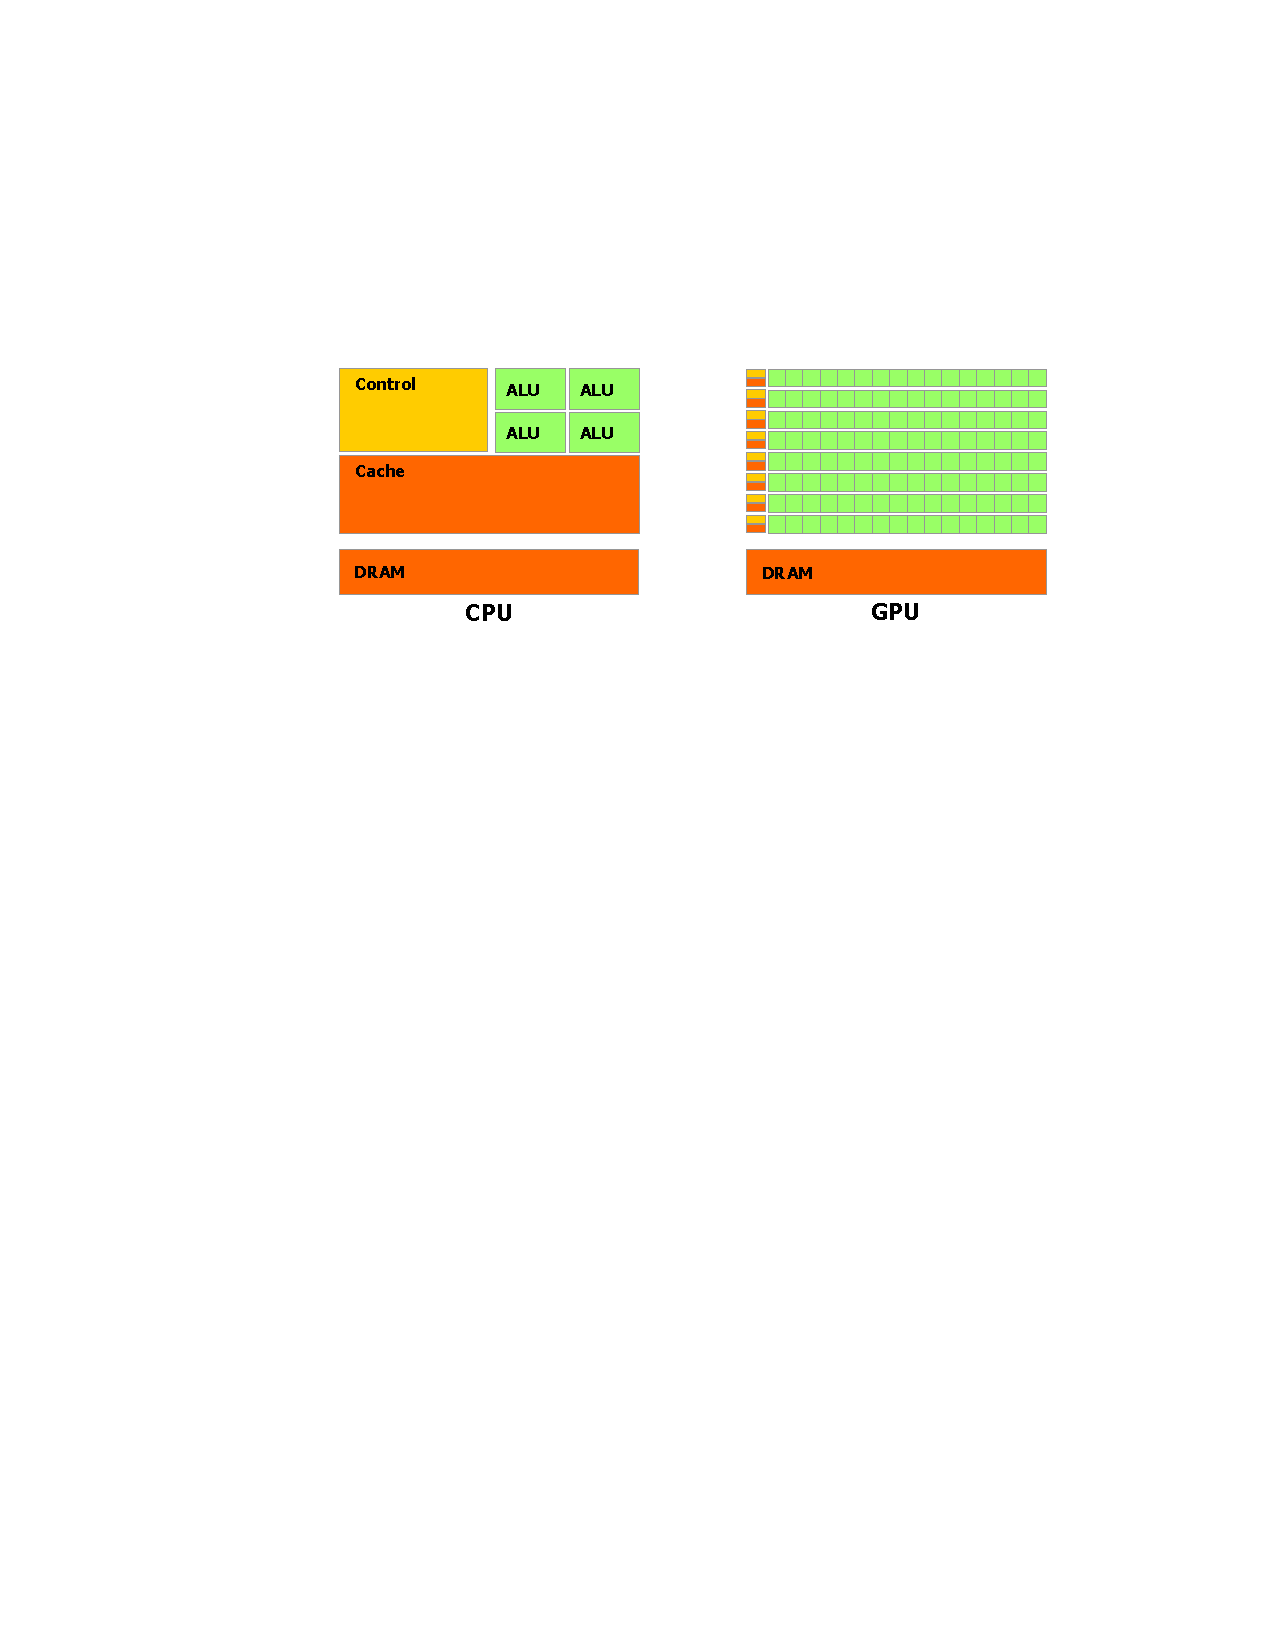
\includegraphics[width=1\textwidth]{images/cpuvsgpu.pdf}
	\caption{Comparativa de organización de CPU y GPU \cite{nvidia:cuda_c_programming_guide}}\label{fig:cudaorggpu}
\end{figure}

Además de como está organizada la GPU, es importante tener en cuenta como se organiza la memoria (figura~\ref{fig:memcuda}) ya que el buen uso de ésta influirá de forma muy significativa en el rendimiento de los programas. Esta arquitectura es la misma que la de las tarjetas gráficas y se puede representar como una pirámide de tiempos dependiendo del tipo de memoria a la que se vaya a acceder.

La memoria de sistema es la que se encuentra en el equipo sin contar la que aporta la tarjeta gráfica. Los programas de ordenador puede hacer uso de ésta de forma sencilla, pero los programas que se ejecutan dentro de la GPU no puede acceder a ella. Tanto la memoria global como la memoria de textura se encuentran en la tarjeta gráfica y servirán de almacén de los datos que requieran los programas que se hallen en ésta. La principal diferencia entre ambas reside en el modo a través del cual se accede a ellas. La memoria global funciona igual que la memoria de sistema para un programa normal (a partir de un puntero se accede a la misma), mientras que la memoria de textura se accede haciendo uso de un sistema especial que añade funcionalidades como la interpolación de los valores. La ventaja de la memoria de textura es que dispone de un acceso más rápido (se debe a que es guardada en caché) lo que la convierte en una opción muy atractiva para cierto tipo de cálculos.

Por último, los registros de la GPU disponen de un acceso muy rápido por lo que es recomendable hacer uso de los mismos siempre que sea posible.

\begin{figure}
	\centering
	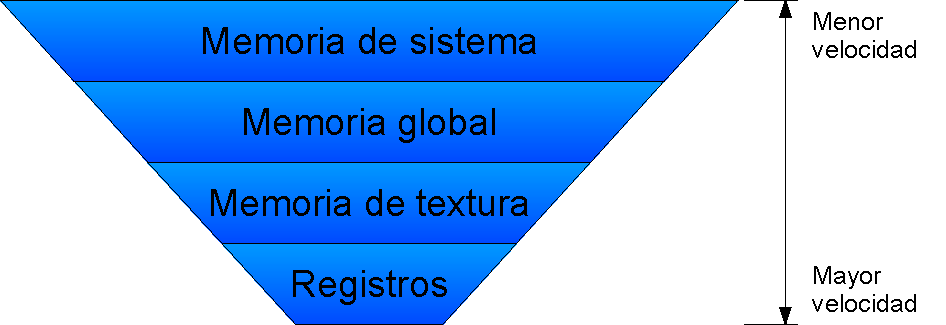
\includegraphics[width=0.7\textwidth]{images/MemoriaCuda.pdf}
	\caption{Jerarquía de memoria en CUDA}\label{fig:memcuda}
\end{figure}

La optimización del uso de la memoria es fundamental para mejorar el rendimiento de las aplicaciones CUDA ya que si se trabaja con una cantidad muy grande de datos se puede perder una parte importante de tiempo realizando copias de memoria. Por este motivo hay que realizar un buen estudio sobre el uso que se va a realizar de la memoria.

\subsection{Modo de desarrollo}

Para programar con CUDA es muy importante tener en cuenta cómo se organiza la ejecución del código ya que influirá en la forma en la que habrá que diseñar nuestros algoritmos. De éste modo, los códigos que se ejecutan en la tarjeta gráfica se organizarán del siguiente modo:

\begin{description}
	\item[\emph{threads}] que son tareas que se ejecutan en paralelo y que comparten código. Los \emph{threads} se organizan de forma tridimensional de tal modo que podría haber momentos en los que un \emph{thread} estuviese encima, debajo o al lado de otro.

	\item[\emph{blocks}] que son grupos de \emph{threads} y, al igual que éstos, también se organizan de forma tridimensional. Todos los \emph{threads} contenidos en un \emph{block} se ejecutarán al mismo tiempo, de modo que si la GPU no tiene capacidad para el total de \emph{threads} solicitados por \emph{block} devolverá un error.

	\item[\emph{grid}] que es un conjunto de \emph{blocks}. Los \emph{grids} se organizan en planos, esto es, solo dispone de 2 dimensiones.
\end{description}

En la figura~\ref{fig:cudaorg} puede verse de forma más clara la organización de los \emph{threads}. Es importante tener en cuenta que, como se ha dicho, todos los \emph{threads} de un \emph{block} se ejecutan a la vez, pero los \emph{blocks} no tienen porque hacerlo. Este detalle es importante a la hora de ajustar el acceso a la memoria ya que cuando un \emph{thread} accede a ésta podrá verse optimizado si lo hace de forma ordenada con el resto de \emph{threads} del \emph{block}.

\begin{figure}
	\centering
	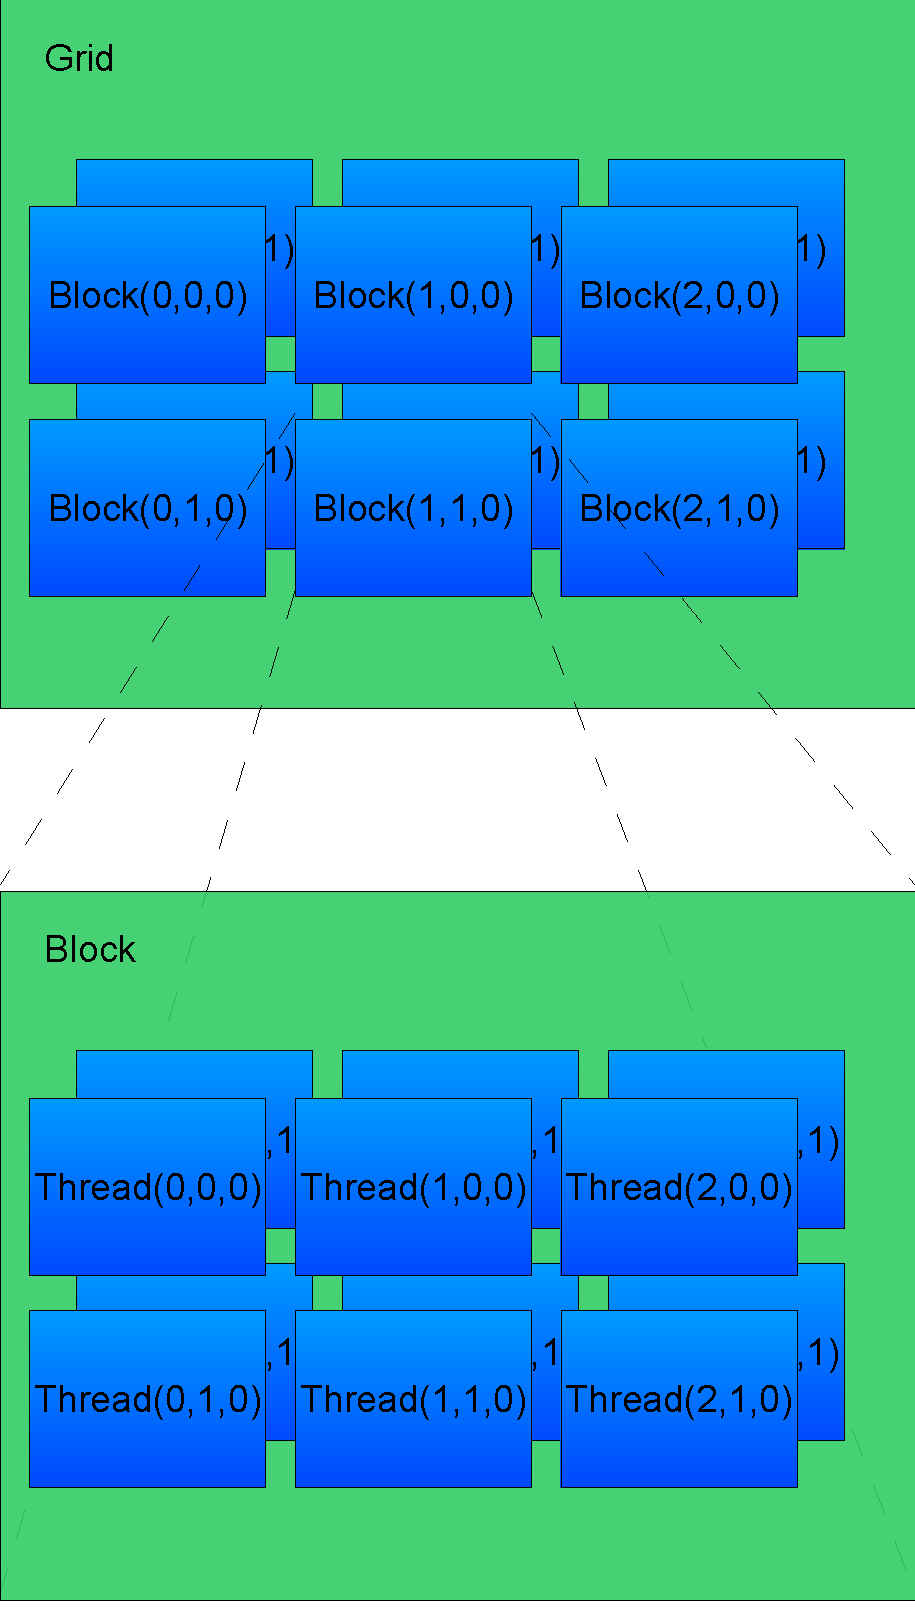
\includegraphics[width=0.7\textwidth]{images/cuda_org.pdf}
	\caption{Organización de procesos en ejecución en CUDA}\label{fig:cudaorg}
\end{figure}

Otro aspecto muy importante a tener en cuenta es la organización del acceso a memoria. Como ya se vio en el apartado anterior, ésta está organizada de forma jerárquica según la velocidad de acceso. Además, también es importante tener en cuenta como los \emph{threads} acceden a la memoria ya que si lo hacen de manera organizada se puede conseguir incrementos de rendimiento. Esto último se debe a que, si por ejemplo todos los \emph{threads} acceden a posiciones contiguas de memoria (el primer \emph{thread} lee el primer elemento de la memoria, el segundo \emph{thread} lee el segundo elemento, etc.) se consigue que todas las lecturas de todos los \emph{threads} se realicen en paralelo. Por el contrario, si las lecturas se hacen de forma desordenada, éstas se realizarán de forma secuencia, malgastando de este modo un tiempo precioso.
 
Como la memoria del sistema es inaccesible para los \emph{threads} es importante tener en cuenta que sólo se podrá utilizar la memoria de la tarjeta gráfica. Esto supone que antes de realizar operaciones sobre memoria en CUDA hay que reservar la memoria a utilizar e inicializarla desde el programa principal que se encuentra en la CPU. Esta inicialización suele realizarse en tres tiempos:

\begin{enumerate}
	\item En un primer momento se preparan los datos que se pasarán a la GPU.

	\item Seguidamente se reserva la memoria en la tarjeta gráfica

	\item Por último se copian los datos a la tarjeta gráfica para poder ser usados desde la parte que será ejecutada en la GPU.
\end{enumerate} 

Por otra parte, hay que tener en cuenta que una vez se disponen de los datos sobre la memoria de la tarjeta gráfica es importante estudiar si conviene utilizarlos desde dicho punto o si es preferible realizar una copia a los registros de la GPU que serán mucho más rápidos. La tarjeta gráfica provee de una gran cantidad de registros (hasta 16.384 en el caso de las NVIDIA Tesla) para poder acelerar los cálculos, por lo que se deberá hacer uso de los mismos, en la medida de lo posible. De este modo, si la cantidad de operaciones a realizar va a ser muy elevada, compensa el tiempo que se dedicará a copiar los datos desde la memoria de la tarjeta gráfica a los registros.

Por norma general, todo código que vaya a ser alojado en una GPU seguirá un patrón de ejecución como el descrito a continuación (figura~\ref{fig:procejecuda}):

\begin{itemize}
	\item Se copian los parámetros que se hallen en memoria global a registros, siempre que sea posible, para acceder a los mismos desde ahí. Esto es especialmente importante si el número de accesos va a ser elevado ya que de otra forma se estaría desperdiciando una gran cantidad de tiempo en realizar accesos a memoria.
	\item Una vez que ya se tiene la memoria iniciada se procede a realizar los cálculos oportunos.
	\item Finalmente se preparan los resultados para ser volcados a la memoria global de la tarjeta gráfica y que de este modo puedan ser leídos por la aplicación.
\end{itemize}

\begin{figure}
	\centering
	
\includegraphics[width=0.7\textwidth]{images/proc_ejec1.pdf}
	\caption{Proceso de ejecución de un algoritmo en CUDA}\label{fig:procejecuda}
\end{figure}

El \emph{kit} de desarrollo de CUDA ofrece dos formas diferentes de desarrollar aplicaciones. En la primera forma, la más sencilla, CUDA se encarga de realizar las llamadas al código que se alojará en la GPU de forma transparente de tal forma que no tendremos que preocuparnos de configurar muchos de los parámetros de los que dispone el sistema. Este mecanismo es muy útil y permite un desarrollo rápido de funciones. Por otra parte estaría el sistema completo con el que debe utilizarse la API de bajo nivel de CUDA y que permite un nivel más alto de granularidad. Con este sistema nosotros deberemos de realizar ``a mano'' la carga del código en la GPU, seleccionar la GPU de todas las posibles, etc.

Con independencia del mecanismo elegido para utilizar CUDA hay algunas tareas que se deben realizar siempre de forma manual. La más importante es la administración de la memoria; cuando se va a enviar datos a la tarjeta gráfica antes de nada hay que reservar la memoria y luego se debe hacer una copia de los datos desde la memoria de sistema a la memoria que se acaba de reservar. Cuando este área de memoria ya no se necesite se deberá liberar.

El proceso de copiar memoria desde la RAM a la tarjeta gráfica es bastante rápido gracias a los nuevos buses de comunicaciones PCI Express que están especialmente diseñados para estas labores, pero esto no evita el hecho de que si la cantidad de datos a copiar es muy grande el tiempo desperdiciado entre llamadas puede ser muy grande. Esto se hace realmente patente cuando el proceso a ejecutar es muy rápido, donde se puede perder mucho tiempo realizando copias de memoria.

Por el motivo anterior CUDA provee de técnicas más avanzadas para optimizar el uso de la arquitectura y mejorar la concurrencia y así evitar tiempos muertos (figura~\ref{fig:cudaejecavanzada}). Éstas consisten en el uso de \emph{streams}, por un lado, y, si es posible, la reutilización de resultados previos. Los \emph{streams} son un mecanismo de comunicación con la tarjeta gráfica que permite tener varios canales de comunicaciones asociados con una llamada a función. Cuando se utiliza \emph{streams} se puede disponer de dos canales, mientras se está ejecutando una función por el primer canal ya se puede utilizar el segundo canal para cargar los datos de la siguiente ejecución. Esto permite optimizar el uso de los tiempo muertos de la CPU y se ahorra la espera de la carga desde memoria de sistema a la memoria de la tarjeta gráfica.

\begin{figure}
	\centering
	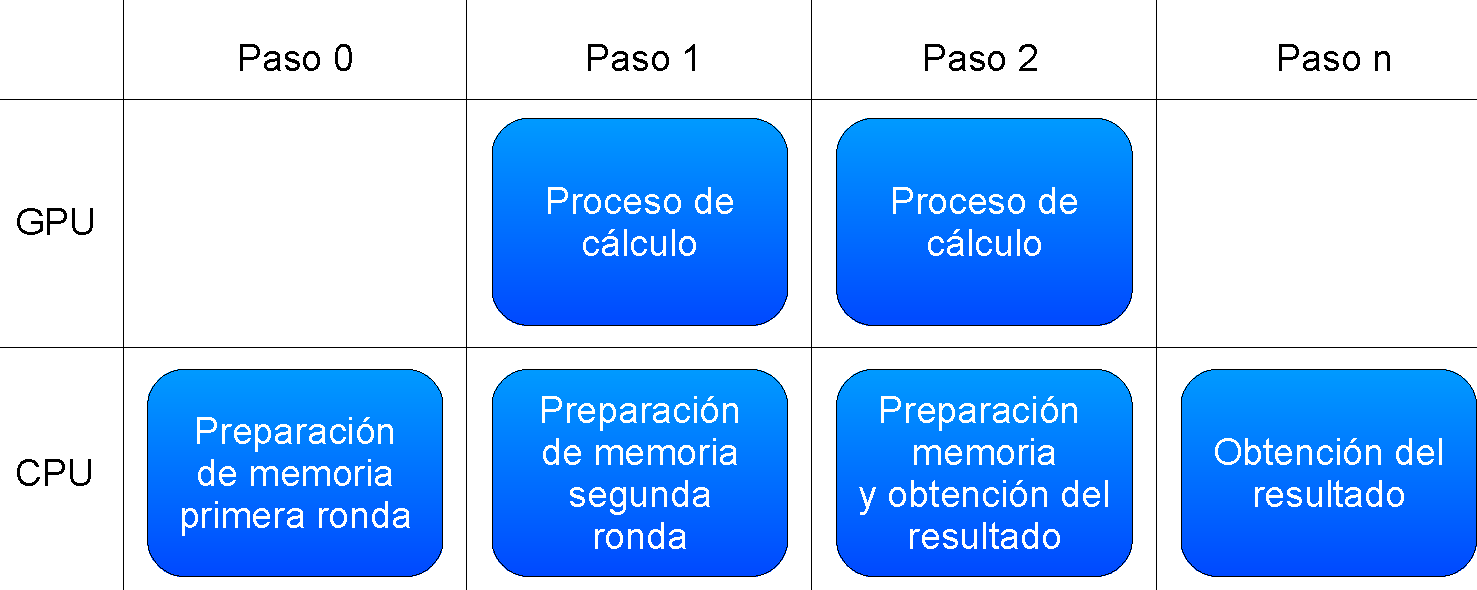
\includegraphics[width=1\textwidth]{images/ejec_gpu_complex.pdf}
	\caption{Ejecución en GPU optimizando usando streams}\label{fig:cudaejecavanzada}
\end{figure}

La reutilización de los valores previos es muy útil cuando se utilizan funciones de la forma $f(x) = af(x-1)+b$ ya que evita tener que realizar un exceso de copias de memoria. Si ya disponemos del resultado de la próxima ejecución en memoria simplemente lo dejamos ahí y lo utilizamos en lugar de copiarlo a la memoria de sistema para después cargarlo a la memoria de la tarjeta gráfica.


